\documentclass[12pt]{article}
\usepackage[margin=1.2in]{geometry}
\usepackage{amsmath}
\usepackage{ctex}
\usepackage{siunitx}
\usepackage{graphicx}
\usepackage{subcaption}
\usepackage{gensymb} 
\usepackage{xcolor}
\usepackage{soul} 
\usepackage{tcolorbox} 
\usepackage{float} 
\newtcolorbox[auto counter, number within=section]{highlightedsection}[2][]{colframe=cyan!80!black, colback=cyan!30, coltitle=black, sharp corners, fonttitle=\bfseries, title=#2,#1}

\title{实验一\,\,Altera FPGA开发入门报告}
\author{姓名：怀迪\,\, 学号：PB23061112 \\ }
\date{}

\begin{document}
\maketitle

% 使用 tcolorbox 使标题带有荧光笔效果
\begin{highlightedsection}{}
    一、设计流程总结
\end{highlightedsection}
本次实验流程较少，我们只需要跟着文档的指示一步一步完成就可以了，
本次实验让我对Quartus软件的使用有了初步的认识。


主要流程如下：
\subsection*{1.创建新工程}
在实验开始前，首先需要创建一个新的工程以保存实验代码以方便不同实验的区分。

打开Quartus软件，点击“File”菜单，
”File”菜单，选择“New…”命令，在弹出的New窗口中选择“New Quartus II Project”项后，单击“OK”按钮然后
点击“NEXT”按钮，选择工程存放的位置以及命名好工程名字之后，再次点击“NEXT”按钮进行
FPGA器件选择后（见下图）
\begin{figure}[H]  % H 表示固定图片位置
    \centering
    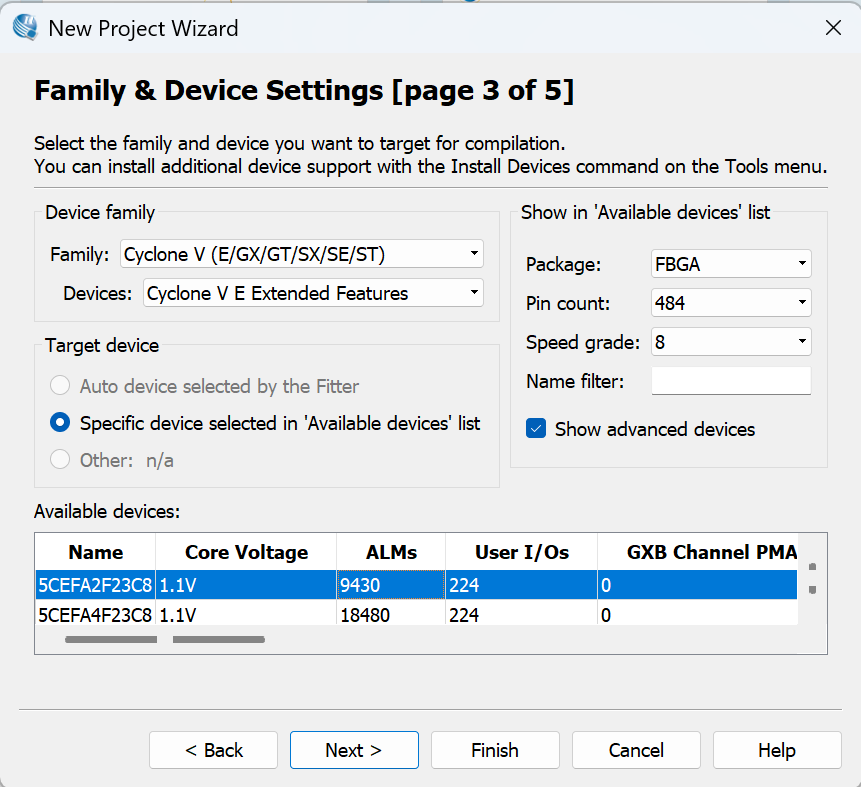
\includegraphics[width=0.5\textwidth]{1.png}  % 图片的最大宽度为文本宽度
\end{figure}
再选择仿真软件和语言分别为""ModelSim"和"Verilog HDL"后，点击“Finish”按钮完成新工程的创建。

\subsection*{2.添加并编写Verilog设计文件及源代码}
创建好工程后，接下来我们就可以在工程里添加我们要编写的Verilog文件了，我们可以电击下图两个按钮
中的任意一个，然后在弹出的New窗口中选择“Verilog HDL File”项，然后单击“OK”按钮。
\begin{figure}[H]  % H 表示固定图片位置
    \centering
    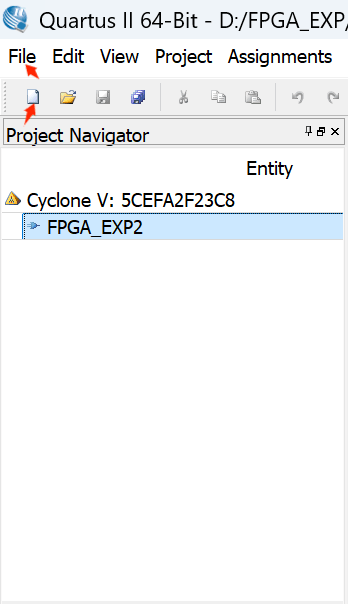
\includegraphics[width=0.6\textwidth]{2.png}  % 图片的最大宽度为文本宽度
\end{figure}

然后就可以在弹出的新窗口中编写Verilog代码了，编写完成后点击"File"->"Save"或者按下图图标->"Save"
进行保存到相应文件夹即可。
\begin{figure}[H]  % H 表示固定图片位置
    \centering
    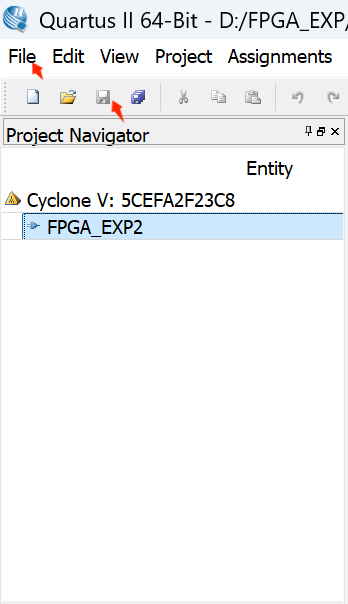
\includegraphics[width=0.6\textwidth]{3.png}  % 图片的最大宽度为文本宽度
\end{figure}



\subsection*{3.对Verilog源代码进行综合与分析}
鼠标左键单击”Processing”菜单，选择“Start”子菜单中的”Start Analysis Synthesis“命令或者
点击下图的图标（个人觉得这种方法更方便一点），完成功能仿真前的分析和综合。
\begin{figure}[H]  % H 表示固定图片位置
    \centering
    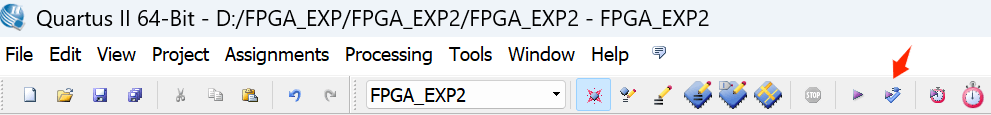
\includegraphics[width=\textwidth]{4.png}  % 图片的最大宽度为文本宽度
\end{figure}
窗口显示没有错误，那么就可以进入下一个流程了。


\subsection*{4.编写测试平台程序，进行仿真，观察仿真结果}
依照步骤2，再次添加仿真文件及源代码，按照步骤2进行保存，
注意文件名应该在设计文件名后加上“tb”，表示这是一个仿真文件，
而后再次进行步骤3。

然后是“ModelSim”仿真工具的设置，单击“Tools”菜单，选择“Options…”命令，在弹
出“Options”窗口的左侧单击”General”下的“EDA Tool Options”，然后按下图设置
右侧 “EDA Tool Options”页面下的“ModelSim-Altera”之“Location of Executable”
为 “\verb|C:\altera\13.1\modelsim_ae\win32aloem\|”
（每个人存放路径不同，实际路径选择也不同）

单击“Assignments”菜单，选择“Settings…”命令，在弹出
“Settings”窗口的左侧单击”EDA Tool Settings”下的“simulation”，然后按下图设置
右侧的“Simulation”参数。

与实验一文档里的设置稍有不同，tool name应选择为“ModelSim-Altera”，否则无法仿真。
\begin{figure}[H]  % H 表示固定图片位置
    \centering
    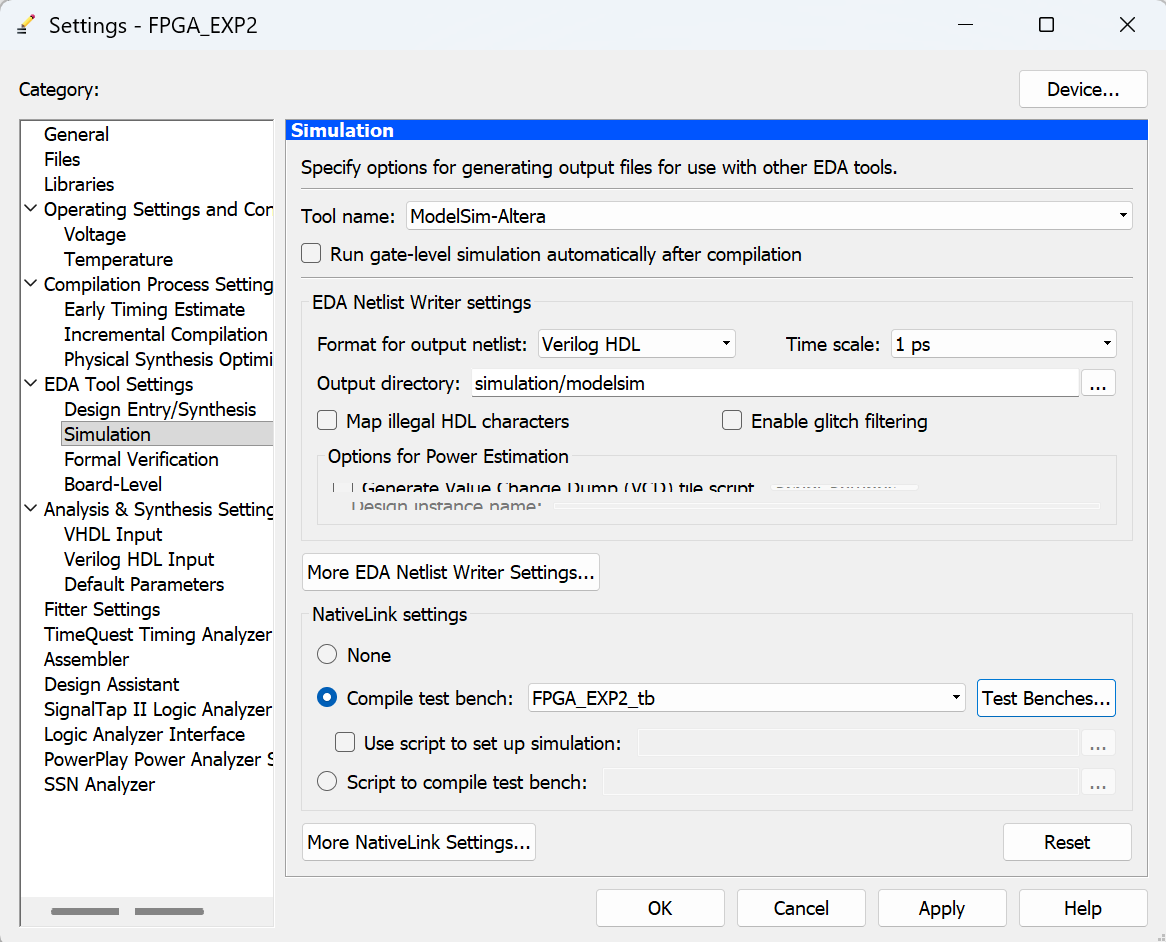
\includegraphics[width=0.7\textwidth]{5.png}  % 图片的最大宽度为文本宽度
\end{figure}
后面就可以启动仿真了，单击“Tools”菜单，选择“Run Simulation 
Tool”子菜单中的“RTL Simulation”命令来启动 Modelsim 实现功能仿真。等待
ModelSim 完全打开并跑完设定的1000 ns，可以看到Modelsim的基本仿真界面
及仿真结果，我的仿真结果如下图所示。
\begin{figure}[H]  % H 表示固定图片位置
    \centering
    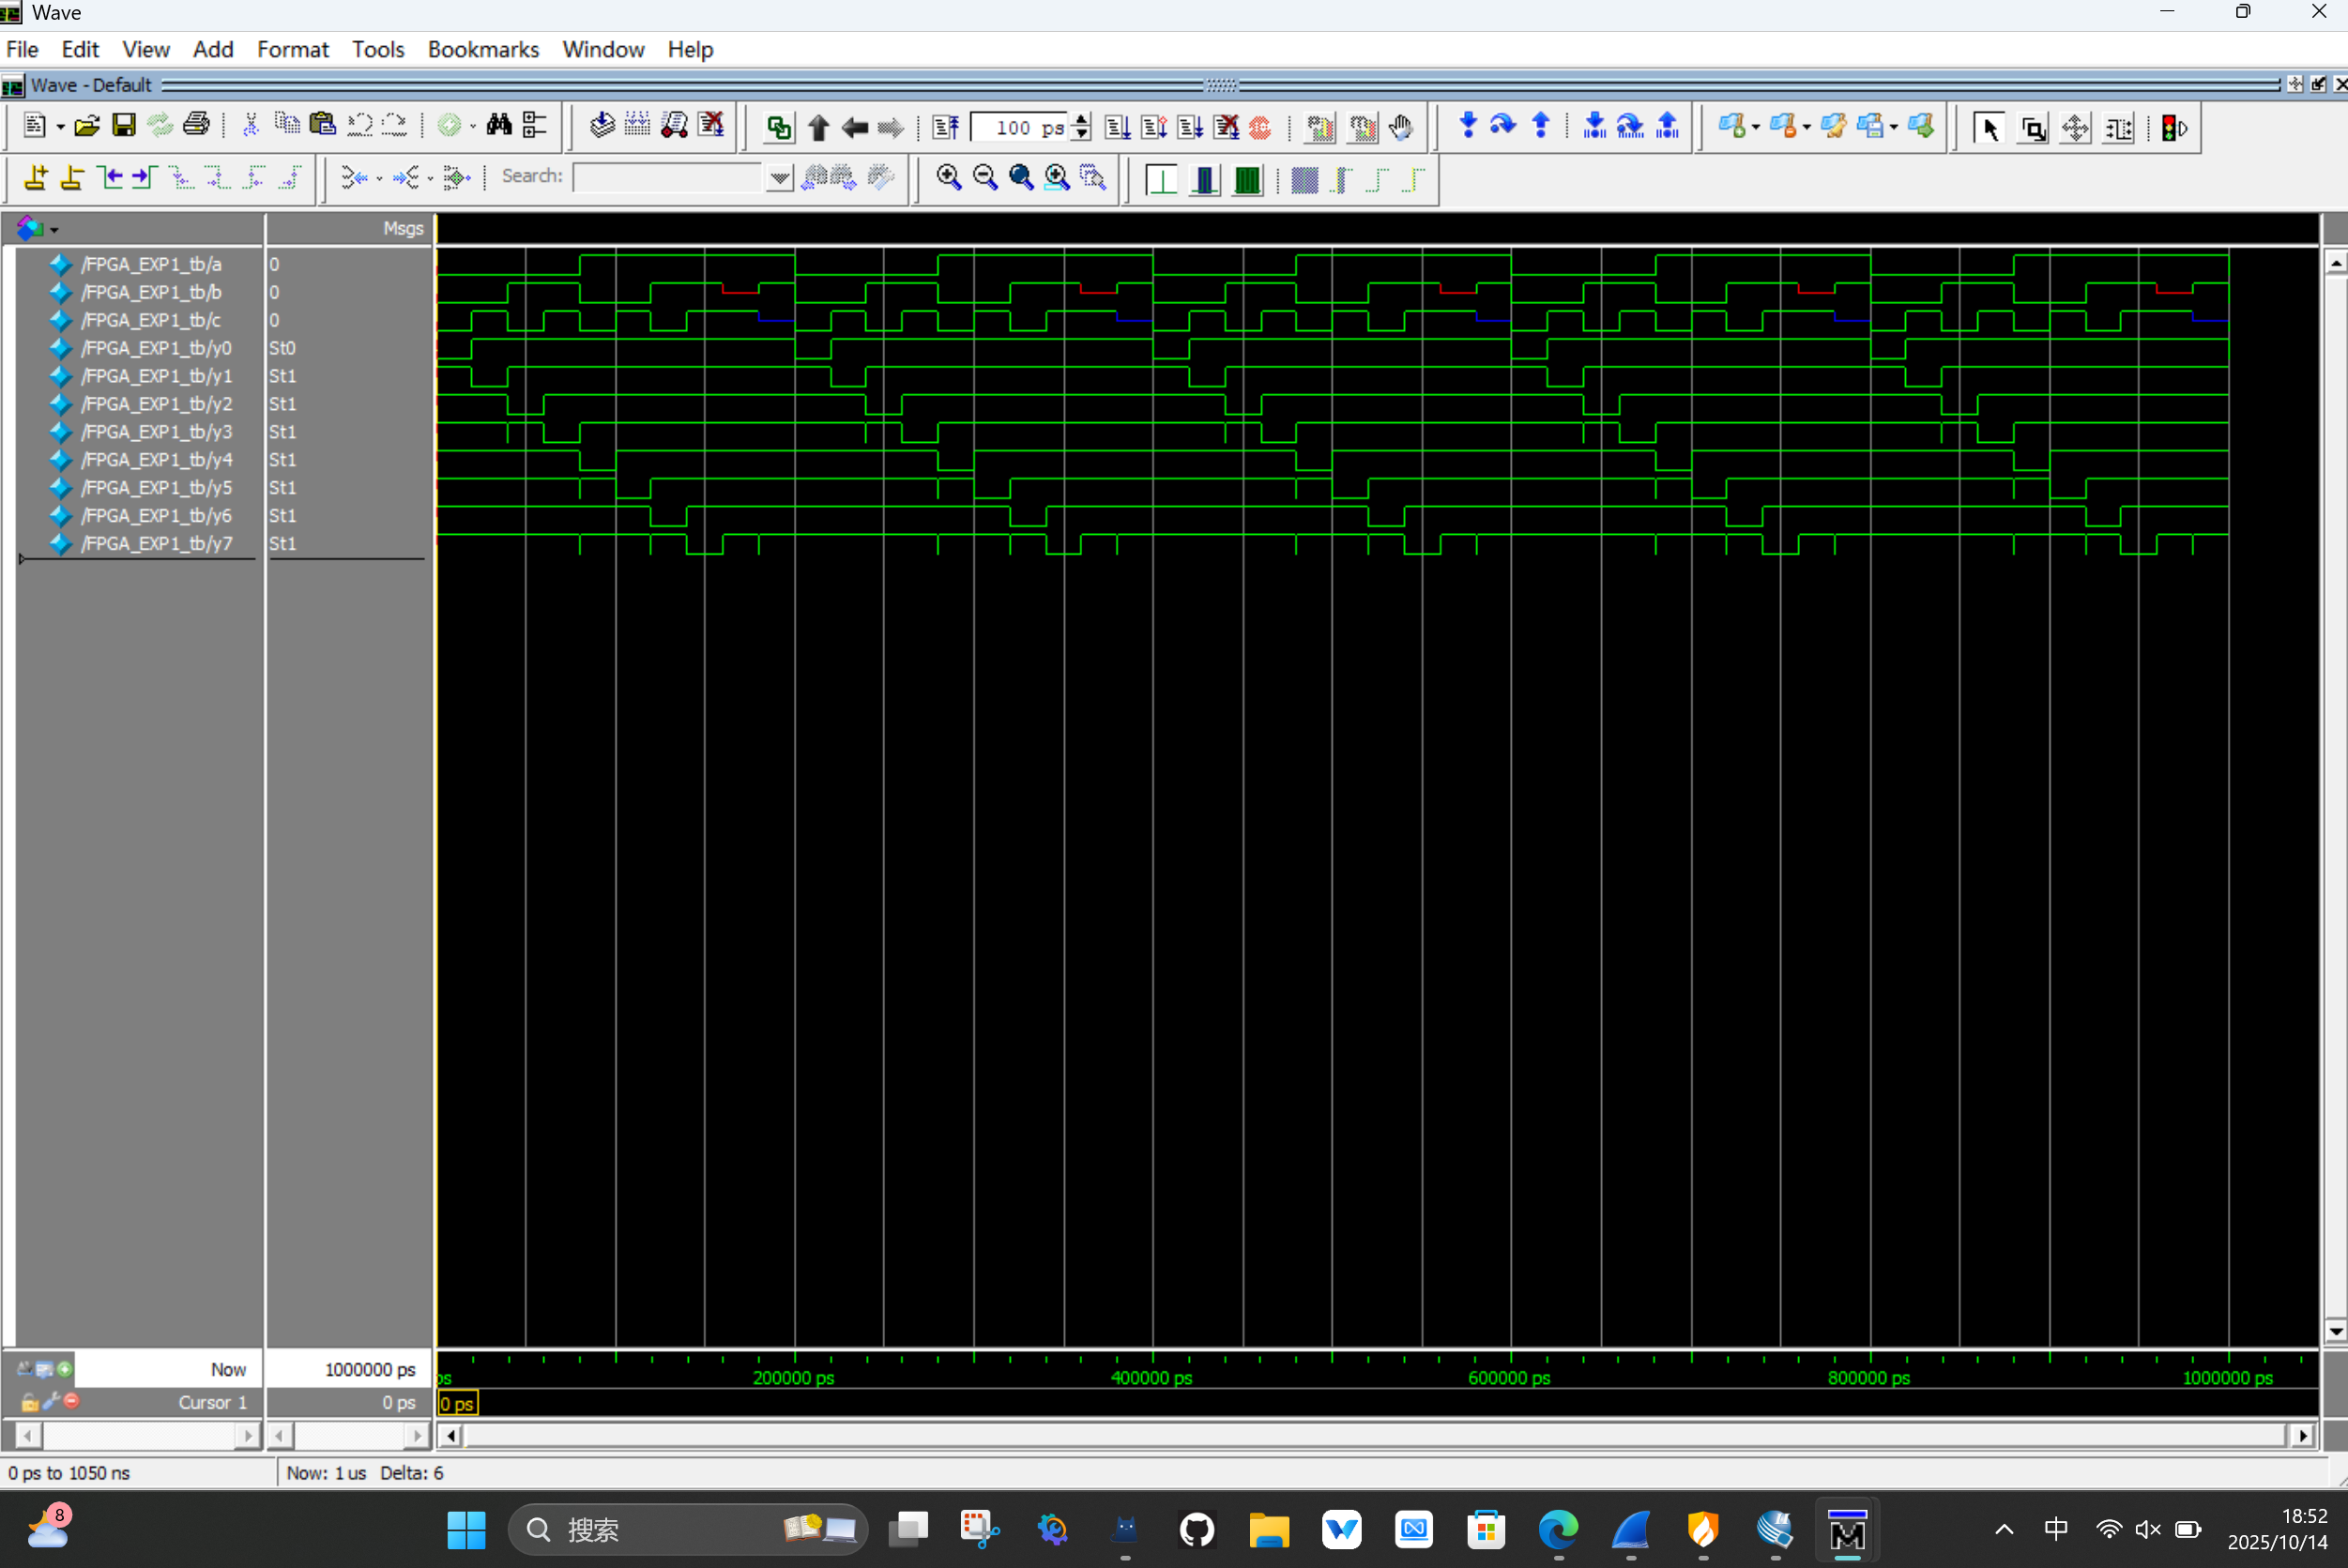
\includegraphics[width=\textwidth]{仿真图.png}  % 图片的最大宽度为文本宽度
\end{figure}
仿真结果与预期相符，说明代码正确，可以进行下一步。


\subsection*{5.为设计工程添加约束：管脚分配}
代码正确后，我们需要为硬件实现进行管脚分配，单击“Assignments”菜单，选择“Pin Planner”命令，
在弹出的“Pin Planner”窗口中进行管脚分配，分配完成后，就可以关闭“Pin Planner”窗口，系统会自动保存管脚分配。
后续如果想要修改引脚，则进行相同的操作即可。

\subsection*{6.进行全编译，生成配置文件}
单击“Processing”菜单，选择“Start Compilation”命令，实现 Analysis
Synthesis、Fitter 及 Assembler 等完整的全编译过程。成功编译后会出现下图中的
提示信息。则说明编译成功，可以进行下一步。
\begin{figure}[H]  % H 表示固定图片位置
    \centering
    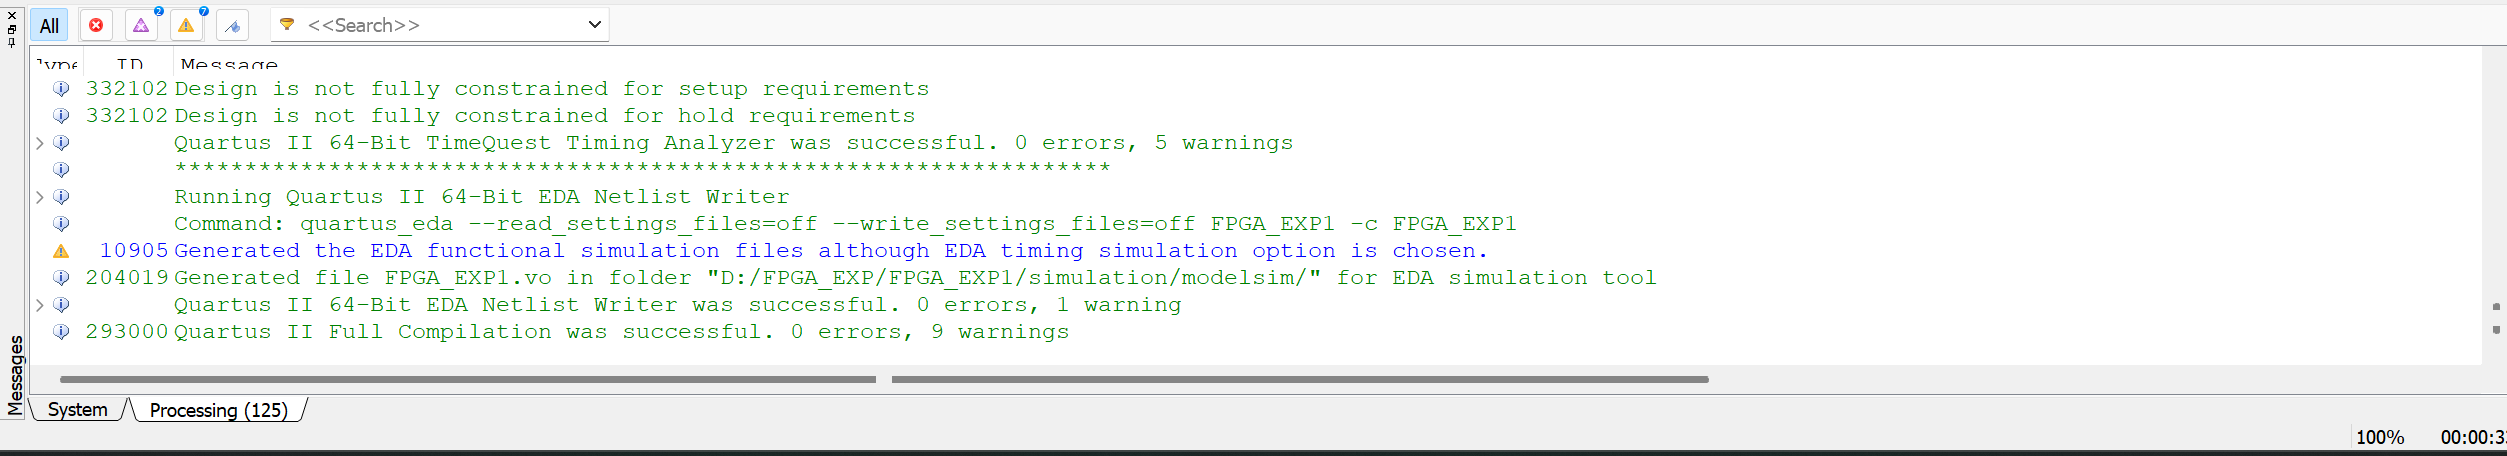
\includegraphics[width=\textwidth]{6.png}  % 图片的最大宽度为文本宽度
\end{figure}

\subsection*{7.硬件验证}
软件上的工作已基本完成，下面只需要连接硬件把代码烧录进去即可进行验证。

用USB-Blaster下载线连接电脑和试验箱，用电源线给试验箱进行供电。

由于是首次实验，故我需要安装USB-Blaster驱动程序，按照文档步骤安装完驱动程序后，
单击”Tools”菜单，选择”Programmer“命令，在打开的”Programmer“窗口中。
单击“Start”按钮把设计电路下载到Altera FPGA实验箱的FPGA芯片5CEFA2F23中，而后即可
拨动试验箱上的按钮进行功能验证。

根据实验文档上的指示，拨动实验箱不同的开关，可以看到不同的LED灯亮起和熄灭，实验成功。

\begin{highlightedsection}{}
    二、实验中出现的体会、问题与解决方案
\end{highlightedsection}
本次实验并不需要太过复杂的操作，只需要跟着实验文档进行操作即可完成实验。

但是在进行仿真时，遇到了一些问题，导致无法进行仿真。
问题主要出现在EDA Tool Settings的设置上，Tool name应选择为“ModelSim-Altera”，
否则无法仿真。

这与实验文档一中的设置稍有不同，文档中选择的是“ModelSim”，所以我们还是需要根据
错误提示进行正确的配置。

本次实验让我对Quartus软件的使用有了初步的认识。期待后续的实验。





\end{document}